% ==========================================================================
% Rapport de soutenance - TP de Régression Logistique
% Institut National de Statistique et d'Économie Appliquée (INSEA)
% ==========================================================================
\documentclass[11pt,a4paper,twoside]{report}

% --------------------------------------------------------------------------
% Encodage et langue
% --------------------------------------------------------------------------
\usepackage[utf8]{inputenc}
\usepackage[T1]{fontenc}
\usepackage[french]{babel}
\usepackage{lmodern}
\usepackage{microtype}

% --------------------------------------------------------------------------
% Mise en page
% --------------------------------------------------------------------------
\usepackage[a4paper,top=2.5cm,bottom=2.5cm,left=2.8cm,right=2.8cm]{geometry}
\usepackage{setspace}
\onehalfspacing
\usepackage{fancyhdr}
\pagestyle{fancy}
\fancyhf{}
\fancyhead[LE,RO]{\thepage}
\fancyhead[RE]{\itshape\leftmark}
\fancyhead[LO]{\itshape\rightmark}
\renewcommand{\headrulewidth}{0.4pt}

% --------------------------------------------------------------------------
% Mathématiques
% --------------------------------------------------------------------------
\usepackage{amsmath,amssymb,amsthm,mathtools}
\usepackage{bm}

% --------------------------------------------------------------------------
% Graphismes / tableaux
% --------------------------------------------------------------------------
\usepackage{graphicx}
\usepackage{float}
\usepackage{booktabs}
\usepackage{multirow}
\usepackage{array}
\usepackage{caption}
\usepackage{subcaption}
\captionsetup{font=small,labelfont=bf}
\usepackage{xcolor}
\definecolor{insea}{RGB}{15,70,120}
\definecolor{accent}{RGB}{210,90,40}
\usepackage[most]{tcolorbox}

% --------------------------------------------------------------------------
% Listings (code Python)
% --------------------------------------------------------------------------
\usepackage{listings}
\lstset{
  basicstyle=\ttfamily\footnotesize,
  keywordstyle=\color{insea}\bfseries,
  commentstyle=\color{gray}\itshape,
  stringstyle=\color{accent},
  showstringspaces=false,
  breaklines=true,
  breakatwhitespace=true,
  language=Python,
  frame=single,
  rulecolor=\color{gray!50},
  numbers=left,
  numberstyle=\tiny\color{gray},
  tabsize=4,
  xleftmargin=15pt
}

% --------------------------------------------------------------------------
% Hyperliens
% --------------------------------------------------------------------------
\usepackage[colorlinks=true,linkcolor=insea,citecolor=insea,urlcolor=accent]{hyperref}

% --------------------------------------------------------------------------
% Commandes personnelles
% --------------------------------------------------------------------------
\newcommand{\OR}{\mathrm{OR}}
\newcommand{\logit}{\mathrm{logit}}
\newcommand{\E}{\mathbb{E}}
\newcommand{\Var}{\mathrm{Var}}
\newcommand{\Prob}{\mathbb{P}}
\DeclareMathOperator*{\argmin}{arg\,min}
\DeclareMathOperator*{\argmax}{arg\,max}

\theoremstyle{definition}
\newtheorem{definition}{Définition}[chapter]
\newtheorem{remarque}{Remarque}[chapter]
\newtheorem{propriete}{Propriété}[chapter]

% ==========================================================================
\begin{document}

% --------------------------------------------------------------------------
% Page de garde
% --------------------------------------------------------------------------
\begin{titlepage}
  \begin{center}
    \vspace*{0.5cm}
    {\large\textsc{Royaume du Maroc}}\\[0.2cm]
    {\large\textsc{Haut-Commissariat au Plan}}\\[0.4cm]
    \rule{\textwidth}{0.5pt}\\[0.3cm]
    {\Large\bfseries Institut National de Statistique et d'Économie Appliquée}\\[0.15cm]
    {\normalsize (INSEA)}\\[0.2cm]
    \rule{\textwidth}{0.5pt}\\[2.5cm]

    {\large \textsc{Rapport de Travaux Pratiques}}\\[0.6cm]
    {\large Module : \emph{Modèle Linéaire Généralisé}}\\[2.5cm]

    \begin{tcolorbox}[colback=insea!8,colframe=insea,arc=4pt,boxrule=1pt]
    \centering
    {\Huge\bfseries\color{insea} Pratique du modèle de régression logistique\\[0.3em]
    sous Python}\\[0.8em]
    {\Large\itshape Application à la prédiction de la maladie cardio-vasculaire}\\[0.4em]
    {\large (Cleveland Heart Disease Dataset)}
    \end{tcolorbox}

    \vfill

    \begin{minipage}{0.45\textwidth}
      \begin{flushleft}
        \textbf{\large Réalisé par :}\\[0.3em]
        M.\ DAOUDI Adam
      \end{flushleft}
    \end{minipage}
    \hfill
    \begin{minipage}{0.45\textwidth}
      \begin{flushright}
        \textbf{\large Encadré par :}\\[0.3em]
        Mme F.\ BADAOUI\\
        Professeure à l'INSEA
      \end{flushright}
    \end{minipage}

    \vspace{1.5cm}
    \rule{\textwidth}{0.5pt}\\
    {\large Année Universitaire 2025--2026}\\[0.3em]
    \textbf{22 avril 2026}
  \end{center}
\end{titlepage}

\newpage\thispagestyle{empty}~\newpage

% --------------------------------------------------------------------------
% Remerciements
% --------------------------------------------------------------------------
\chapter*{Remerciements}
\addcontentsline{toc}{chapter}{Remerciements}

Je tiens à exprimer ma profonde gratitude à \textbf{Mme Fadoua BADAOUI},
professeure à l'INSEA, pour la qualité de son enseignement du module
\emph{Modèle Linéaire Généralisé} et pour la rigueur théorique avec
laquelle elle a présenté cette matière essentielle à la formation
statistique. Son polycopié détaillé a constitué la référence principale
de ce travail.

Je remercie également l'ensemble du corps pédagogique de l'INSEA pour
leur engagement au service de la formation de statisticiens rigoureux.

Enfin, je remercie la communauté scientifique open-source --- en
particulier les mainteneurs de \texttt{statsmodels}, \texttt{scikit-learn},
\texttt{pandas} et \texttt{matplotlib} --- dont les outils ont permis de
transposer en Python la démarche de modélisation enseignée en R.

% --------------------------------------------------------------------------
% Résumé
% --------------------------------------------------------------------------
\chapter*{Résumé}
\addcontentsline{toc}{chapter}{Résumé}

Ce rapport présente l'application d'un \textbf{Modèle Linéaire Généralisé
Binomial avec fonction de lien logit} (régression logistique) à la
prédiction de la maladie coronarienne sur le jeu de données
\emph{Cleveland Heart Disease} de l'UCI ML Repository (Detrano et al.,
1989). Après une revue des fondements théoriques des GLM --- famille
exponentielle, estimation par maximum de vraisemblance via l'algorithme
IRLS, tests de Wald et de rapport de vraisemblance, déviance, test
d'Hosmer--Lemeshow, diagnostic par les résidus --- la démarche
d'analyse du cours (Mme Badaoui, INSEA, 2026) est appliquée pas à pas.

L'échantillon de 297 patients est découpé de manière stratifiée en 80\,\%
d'apprentissage et 20\,\% de validation. Une sélection \emph{backward} sur
le critère AIC aboutit à un modèle à 8 variables explicatives dominé
cliniquement par le type de douleur thoracique (OR\,$= 6{,}8$), la
thalassémie réversible (OR\,$= 5{,}6$), le nombre de vaisseaux
coronariens atteints (OR\,$= 2{,}5$) et la dépression du segment ST
induite par l'effort (OR\,$= 1{,}9$). Le modèle satisfait l'ensemble des
tests d'adéquation (Hosmer--Lemeshow $p = 0{,}61$, ratio
$D/\mathrm{ddl} = 0{,}74$) et atteint une \textbf{précision de 81,7\,\%}
et une \textbf{AUC de 0,942} sur l'échantillon de validation.

\bigskip
\noindent\textbf{Mots-clés :} modèle linéaire généralisé, régression
logistique, famille exponentielle, maximum de vraisemblance, déviance,
test d'Hosmer--Lemeshow, odds ratio, courbe ROC, Python, statsmodels.

% --------------------------------------------------------------------------
% Tables
% --------------------------------------------------------------------------
\tableofcontents
\listoffigures
\addcontentsline{toc}{chapter}{Table des figures}
\listoftables
\addcontentsline{toc}{chapter}{Liste des tableaux}

\cleardoublepage

% ==========================================================================
\chapter{Introduction}
% ==========================================================================

\section{Contexte}

L'étude quantitative du lien entre une variable à expliquer $Y$ et un
ensemble de variables explicatives $X_1,\ldots,X_p$ est l'objet central
de la \emph{modélisation statistique}. Lorsque la variable réponse est
continue, à valeurs réelles et approximativement distribuée selon une
loi normale, le \textbf{modèle linéaire classique} (régression multiple,
analyse de la variance, analyse de la covariance) constitue l'outil de
référence. Il fait les hypothèses fortes suivantes :

\begin{enumerate}\itemsep0.2em
  \item \textbf{Linéarité} : $\E(Y) = X^\top\beta$ (forme paramétrique) ;
  \item \textbf{Normalité} : $\varepsilon = Y - X^\top\beta \sim \mathcal{N}(0,\sigma^2)$ ;
  \item \textbf{Homoscédasticité} : $\Var(\varepsilon) = \sigma^2$ constante ;
  \item \textbf{Indépendance} des observations.
\end{enumerate}

Or dans de nombreuses situations pratiques, la variable réponse ne
respecte pas ces hypothèses :

\begin{itemize}\itemsep0.2em
  \item \emph{Variables binaires} : présence/absence d'une maladie,
    succès/échec d'un traitement, achat/non-achat d'un produit.
  \item \emph{Variables de comptage} : nombre de sinistres, nombre
    d'appels téléphoniques, nombre de consultations médicales.
  \item \emph{Variables positives dissymétriques} : durée de vie, temps
    d'attente, montant de sinistres.
\end{itemize}

Pour de telles situations, \textbf{Nelder et Wedderburn} ont introduit
en 1972~\cite{nelder} le cadre unifié des \emph{Modèles Linéaires
Généralisés} (GLM, \emph{Generalized Linear Models}), qui étend le
modèle linéaire classique via :

\begin{enumerate}\itemsep0.2em
  \item une \textbf{composante aléatoire} de loi appartenant à la
    \emph{famille exponentielle} (Bernoulli, Binomiale, Poisson, Gamma,
    Normale, etc.) ;
  \item une \textbf{composante déterministe} $\eta = X^\top\beta$, dite
    \emph{prédicteur linéaire} ;
  \item une \textbf{fonction de lien} $g(\cdot)$ monotone et dérivable
    telle que $g\!\big(\E(Y)\big) = \eta$.
\end{enumerate}

Le cas particulier d'une variable réponse binaire avec lien logit
constitue la \textbf{régression logistique}, qui fait l'objet de ce TP.

\section{Objectifs du travail}

Ce rapport poursuit trois objectifs complémentaires :

\begin{enumerate}\itemsep0.3em
  \item \textbf{Objectif pédagogique :} appliquer l'ensemble des étapes
    de modélisation enseignées dans le cours (analyse descriptive,
    échantillonnage stratifié, ajustement par maximum de vraisemblance,
    tests d'hypothèses, adéquation, diagnostic des résidus, comparaison
    de modèles) sur un cas d'étude concret.

  \item \textbf{Objectif opérationnel :} démontrer que la démarche
    théorique présentée en R peut être reproduite \emph{à l'identique} en
    Python via la bibliothèque \texttt{statsmodels}, dont la fonction
    \texttt{GLM} fournit une sortie directement comparable à la fonction
    \texttt{glm()} de R.

  \item \textbf{Objectif scientifique :} construire un modèle prédictif
    interprétable de la maladie coronarienne en identifiant les facteurs
    de risque statistiquement significatifs, dans un esprit
    \emph{d'evidence-based medicine}.
\end{enumerate}

\section{Organisation du rapport}

Ce rapport est structuré en six chapitres :

\begin{itemize}\itemsep0.2em
  \item Le \textbf{Chapitre~2} formalise la problématique médicale et
    justifie le choix d'un modèle logistique.
  \item Le \textbf{Chapitre~3} détaille le cadre théorique du GLM
    logistique tel que présenté dans le cours : famille exponentielle,
    fonction de lien canonique, vraisemblance, tests, adéquation.
  \item Le \textbf{Chapitre~4} présente la méthodologie mise en œuvre :
    source des données, prétraitement, outils logiciels, protocole
    expérimental.
  \item Le \textbf{Chapitre~5} expose les résultats obtenus
    (estimation, tests, diagnostic, validation) et discute leur
    interprétation clinique.
  \item Le \textbf{Chapitre~6} conclut en synthétisant les apports et
    les limites du travail.
  \item L'\textbf{Annexe} fournit le code Python complet utilisé pour
    reproduire l'ensemble des résultats.
\end{itemize}

% ==========================================================================
\chapter{Problématique et choix du cas d'étude}
% ==========================================================================

\section{Contexte épidémiologique}

Les maladies cardio-vasculaires (MCV) constituent la \textbf{première
cause de mortalité mondiale} selon l'Organisation Mondiale de la Santé,
avec environ 17,9 millions de décès annuels. Parmi elles, la
\emph{maladie coronarienne} (Coronary Heart Disease, CHD) représente à
elle seule près de 50\,\% de ces décès.

L'un des enjeux majeurs de santé publique est l'\textbf{identification
précoce des patients à risque} à partir de variables mesurables lors
d'une consultation cardiologique standard : données démographiques
(âge, sexe), mesures physiologiques (pression artérielle, fréquence
cardiaque maximale), résultats d'examens sanguins (cholestérol,
glycémie) et résultats d'examens fonctionnels (électrocardiogramme,
test d'effort, fluoroscopie).

\section{Formulation de la problématique}

\begin{center}
\fbox{\begin{minipage}{0.94\textwidth}\small
\textbf{Problématique :} \\
À partir d'un ensemble de variables cliniques disponibles lors d'une
consultation de routine, est-il possible de construire un modèle
statistique qui :
\begin{itemize}
  \item prédit \emph{avec une bonne précision} la probabilité qu'un
    patient soit atteint d'une maladie coronarienne ;
  \item identifie les \emph{facteurs de risque statistiquement
    significatifs} ;
  \item fournit une \emph{interprétation clinique directement
    exploitable} ?
\end{itemize}
\end{minipage}}
\end{center}

\section{Justification du choix de la régression logistique}

Plusieurs familles de modèles auraient pu répondre à cette question
(arbres de décision, forêts aléatoires, réseaux de neurones, machines à
vecteurs de support). Le choix s'est porté sur la \textbf{régression
logistique} pour les raisons suivantes, alignées avec les besoins
cliniques :

\begin{enumerate}
  \item \textbf{Cohérence avec le cadre du cours.} Le TP demande
    l'application d'un GLM, dont la régression logistique est le
    représentant naturel pour une variable réponse binaire.

  \item \textbf{Interprétabilité.} Les coefficients du modèle
    logistique se transforment en \emph{odds ratios} (OR) via
    $\OR_j = e^{\beta_j}$, lecture universellement utilisée en
    épidémiologie et en médecine factuelle.

  \item \textbf{Assomptions probabilistes claires.} Le modèle produit
    une \emph{vraie probabilité} $\pi(x) \in [0,1]$, pas seulement un
    score, ce qui autorise la comparaison à un seuil de décision
    médicale explicite.

  \item \textbf{Inférence fréquentiste complète.} Disponibilité
    d'intervalles de confiance asymptotiques, de tests de Wald et de
    rapport de vraisemblance, d'outils d'adéquation (déviance,
    Hosmer--Lemeshow), d'analyse des résidus.

  \item \textbf{Robustesse.} Peu de paramètres à estimer, résultats
    stables même avec un effectif modeste (quelques centaines de
    patients), pas de nécessité de \emph{tuning} d'hyperparamètres.
\end{enumerate}

% ==========================================================================
\chapter{Fondements théoriques du GLM logistique}
% ==========================================================================

Ce chapitre résume les éléments théoriques du cours
(Mme F.\ Badaoui, INSEA, 2026)~\cite{cours} indispensables à la
compréhension des choix méthodologiques effectués dans le présent
travail.

\section{La famille exponentielle}

\begin{definition}[Famille exponentielle]
Une loi de probabilité de paramètres $(\theta,\varphi)$ appartient à la
\emph{famille exponentielle} si sa densité s'écrit sous la forme
\begin{equation}
  f(y;\theta,\varphi) \;=\; \exp\!\left\{
    \frac{y\theta - b(\theta)}{a(\varphi)}
    + c(y,\varphi) \right\},
  \label{eq:expfam}
\end{equation}
où $a(\cdot)$, $b(\cdot)$, $c(\cdot)$ sont des fonctions connues, $b$
deux fois dérivable et $b'$ inversible. Le paramètre $\theta$ est dit
\emph{naturel} ou \emph{canonique}, et $\varphi$ est un paramètre de
\emph{dispersion} ou de \emph{nuisance}.
\end{definition}

\begin{propriete}[Moments d'une loi de la famille exponentielle]
Si $Y$ suit la loi donnée par \eqref{eq:expfam}, alors
\begin{align}
  \E(Y)  &= \mu = b'(\theta), \\
  \Var(Y) &= b''(\theta)\, a(\varphi).
\end{align}
\end{propriete}

\paragraph{Cas de la loi de Bernoulli.}
Pour $Y \sim \mathcal{B}(\pi)$, $\Prob(Y=y) = \pi^y(1-\pi)^{1-y}$, on peut
réécrire :
\[
  f(y;\pi) = \exp\!\left\{ y\log\!\frac{\pi}{1-\pi} + \log(1-\pi)\right\},
\]
d'où l'identification :
\[
  \theta = \log\!\frac{\pi}{1-\pi} = \logit(\pi),\qquad
  b(\theta) = \log(1+e^\theta), \qquad a(\varphi)=1.
\]
Le \emph{paramètre canonique} de la loi Bernoulli est donc le
\textbf{logit} de la probabilité de succès, ce qui justifie
théoriquement le choix de cette fonction de lien.

\section{Définition du GLM logistique}

Soient $(Y_i, X_i)_{i=1,\ldots,n}$ un échantillon de $n$ observations,
avec $X_i = (X_{i,1},\ldots,X_{i,p})^\top$. Un GLM logistique suppose :

\begin{equation}
  \left\{
  \begin{aligned}
    Y_i \mid X_i &\;\sim\; \mathcal{B}\big(\pi(x_i)\big),\\
    \logit\big(\pi(x_i)\big) &= \log\frac{\pi(x_i)}{1-\pi(x_i)}
    = \beta_0 + \sum_{j=1}^p \beta_j x_{i,j}.
  \end{aligned}\right.
  \label{eq:glmlogit}
\end{equation}

La fonction de réponse (inverse du lien) est la \emph{sigmoïde} :
\begin{equation}
  \pi(x) \;=\; \frac{\exp(X^\top\beta)}{1+\exp(X^\top\beta)}
  \;\in\; ]0;1[.
\end{equation}

\begin{remarque}
Alternativement, on peut utiliser d'autres fonctions de lien comme le
\emph{probit} $g(\mu) = \Phi^{-1}(\mu)$ ou le \emph{complementary
log-log} $g(\mu) = \log\!\big(-\log(1-\mu)\big)$. Le logit reste
cependant le lien canonique et offre la meilleure interprétabilité.
\end{remarque}

\section{Estimation par maximum de vraisemblance}

La log-vraisemblance du modèle s'écrit :
\begin{align}
  \ell(\beta) &= \sum_{i=1}^n \Big[ y_i \log\pi(x_i) + (1-y_i)\log\big(1-\pi(x_i)\big)\Big] \nonumber \\
  &= \sum_{i=1}^n \Big[ y_i \, X_i^\top\beta - \log\!\big(1+e^{X_i^\top\beta}\big)\Big].
  \label{eq:loglik}
\end{align}

Le gradient (\emph{score}) est :
\begin{equation}
  \nabla\ell(\beta) = \sum_{i=1}^n X_i\big(y_i - \pi(x_i)\big).
\end{equation}

Les équations de vraisemblance $\nabla\ell(\beta) = 0$ sont
\emph{non linéaires} en $\beta$ : il n'existe pas de solution
explicite. On a recours à l'algorithme \textbf{IRLS (Iterated Reweighted
Least Squares)}, équivalent d'une méthode de Newton-Raphson sur
l'information de Fisher :
\begin{equation}
  \beta^{(t+1)} = \beta^{(t)} + \big[I(\beta^{(t)})\big]^{-1} \nabla\ell(\beta^{(t)}),
\end{equation}
où la matrice d'information de Fisher vaut
\begin{equation}
  I(\beta) = X^\top W X, \qquad
  W = \mathrm{diag}\!\big(\pi_i(1-\pi_i)\big).
\end{equation}

\begin{propriete}[Propriétés asymptotiques du MLE]
Sous des conditions de régularité, l'estimateur du maximum de
vraisemblance $\hat\beta$ est convergent, asymptotiquement sans biais,
et
\begin{equation}
  \sqrt{n}\,(\hat\beta - \beta)
  \;\xrightarrow[n\to\infty]{\mathcal{L}}\;
  \mathcal{N}\!\big(0, I^{-1}(\beta)\big).
\end{equation}
\end{propriete}

\section{Tests d'hypothèses}

\subsection{Test de Wald (individuel)}

Pour tester $H_0 : \beta_j = 0$ contre $H_1 : \beta_j \neq 0$,
\begin{equation}
  Z_j = \frac{\hat\beta_j}{\hat\sigma_{\hat\beta_j}}
  \;\xrightarrow[H_0]{\mathcal{L}}\; \mathcal{N}(0,1),
  \qquad
  W_j = Z_j^2 \;\xrightarrow[H_0]{\mathcal{L}}\; \chi^2_1.
\end{equation}

\subsection{Test du rapport de vraisemblance (TRV)}

Soient $M_0 \subset M_1$ deux modèles emboîtés. Sous
$H_0 = \{M_0\}$, la statistique
\begin{equation}
  T = -2\log\frac{L(\hat\beta_0)}{L(\hat\beta_1)}
    = 2\big[\ell(\hat\beta_1) - \ell(\hat\beta_0)\big]
    = D_0 - D_1
  \;\xrightarrow[H_0]{\mathcal{L}}\; \chi^2_{p_1 - p_0}.
\end{equation}

\subsection{Intervalles de confiance}

Un IC asymptotique de niveau $1-\alpha$ pour $\beta_j$ est :
\begin{equation}
  \mathrm{IC}_{1-\alpha}(\beta_j) = \hat\beta_j \pm z_{1-\alpha/2}\,\hat\sigma_{\hat\beta_j},
\end{equation}
et pour l'odds ratio $\OR_j = e^{\beta_j}$ :
\begin{equation}
  \mathrm{IC}_{1-\alpha}(\OR_j) = \exp\!\Big(\hat\beta_j \pm z_{1-\alpha/2}\,\hat\sigma_{\hat\beta_j}\Big).
\end{equation}

\section{Adéquation du modèle}

\subsection{Déviance}

\begin{definition}[Déviance]
Soit $\ell_{\text{sat}}$ la log-vraisemblance du \emph{modèle saturé}
($n$ paramètres, $\hat\mu_i = y_i$). La \emph{déviance} du modèle
ajusté est :
\begin{equation}
  D = 2\big(\ell_{\text{sat}} - \ell_{\hat\beta}\big)
    = 2\sum_{i=1}^n\left\{ y_i\log\!\frac{y_i}{\hat\mu_i}
      + (1-y_i)\log\!\frac{1-y_i}{1-\hat\mu_i}\right\}.
\end{equation}
\end{definition}

Sous l'hypothèse d'adéquation, $D \sim \chi^2_{n-p-1}$ (asymptotique).
Le modèle est jugé satisfaisant si $D / \mathrm{ddl} \lesssim 1$.

\subsection{Statistique du $\chi^2$ de Pearson}

\begin{equation}
  \chi^2_P = \sum_{i=1}^n \frac{(y_i - \hat\mu_i)^2}{\hat\mu_i(1-\hat\mu_i)}
  \;\sim\; \chi^2_{n-p-1}.
\end{equation}

\subsection{Test d'Hosmer--Lemeshow}

\emph{Recommandé dans le cours (p.~104) pour des données binaires
individuelles.} Les probabilités prédites $\hat\pi_i$ sont ordonnées et
partitionnées en $K = 10$ groupes de taille approximativement égale.
Pour chaque groupe $k$, on note $m_k$ l'effectif, $o_k$ le nombre de
succès observés, $\bar\mu_k$ la moyenne des $\hat\pi$. La statistique
\begin{equation}
  C^2 = \sum_{k=1}^K \frac{(o_k - m_k\bar\mu_k)^2}{m_k\bar\mu_k(1-\bar\mu_k)}
  \;\xrightarrow[H_0]{\mathcal{L}}\; \chi^2_{K-2}
\end{equation}
permet de tester l'adéquation : on \emph{conserve} $H_0$
(modèle adéquat) si $p$-value $> 0{,}05$.

\subsection{Pseudo-$R^2$, AIC et BIC}

\begin{equation}
  \text{Pseudo-}R^2 = \frac{D_0 - D}{D_0}, \quad
  \mathrm{AIC} = -2\ell(\hat\beta) + 2p, \quad
  \mathrm{BIC} = -2\ell(\hat\beta) + p\log(n).
\end{equation}

\section{Diagnostic par les résidus}

\subsection{Résidus de Pearson et de déviance}

\begin{equation}
  r_i^P = \frac{y_i - \hat\mu_i}{\sqrt{\hat\mu_i(1-\hat\mu_i)}},
  \quad
  r_i^D = \mathrm{signe}(y_i - \hat\mu_i)\sqrt{d_i},
\end{equation}
où $d_i$ est la contribution individuelle à la déviance. Une
observation telle que $|r_i| > 2$ mérite attention.

\subsection{Leviers et distances de Cook}

Le \emph{levier} $h_{ii}$ est le $i$-ème terme diagonal de la matrice
$H = X(X^\top W X)^{-1}X^\top W$. Un point est influent si
$h_{ii} > 2(p+1)/n$. La \emph{distance de Cook} mesure l'impact global
sur les coefficients :
\begin{equation}
  D_i \;\approx\; \frac{(r_i^P)^2\,h_{ii}}{p(1-h_{ii})^2}.
\end{equation}
Alerte si $D_i > 1$.

\section{Interprétation : \emph{odds ratio}}

Pour une variable binaire $X_j$ et des autres covariables fixées :
\begin{equation}
  \OR_j = \frac{\mathrm{odds}(X_j = 1)}{\mathrm{odds}(X_j = 0)}
        = \exp(\beta_j).
\end{equation}
$\OR > 1$ indique un \emph{facteur de risque} ; $\OR < 1$ un
\emph{facteur protecteur}. Pour une variable continue, $\OR_j$
représente la multiplication de la cote par $e^{\beta_j}$ pour une
augmentation d'une unité de $X_j$.

% ==========================================================================
\chapter{Méthodologie et données}
% ==========================================================================

\section{Source et description des données}

Le jeu de données est le célèbre \textbf{Cleveland Heart Disease
Dataset} de l'UCI Machine Learning Repository~\cite{uci}, issu des
travaux cliniques de Detrano \textit{et al.}\,~\cite{detrano}. Il
rassemble \textbf{303 patients} de la \emph{Cleveland Clinic Foundation}
caractérisés par 13 variables cliniques plus une variable cible.

\subsection{Dictionnaire des variables}

\begin{table}[H]
\centering
\caption{Description des variables du jeu Cleveland Heart Disease}
\label{tab:variables}
\small
\begin{tabular}{lll}
\toprule
\textbf{Variable} & \textbf{Type} & \textbf{Description} \\
\midrule
\texttt{age}      & Quantitative       & Âge du patient (années) \\
\texttt{sex}      & Qualitative (2)    & Sexe : Masculin / Féminin \\
\texttt{cp}       & Qualitative (4)    & Type de douleur thoracique \\
\texttt{trestbps} & Quantitative       & Pression artérielle au repos (mm\,Hg) \\
\texttt{chol}     & Quantitative       & Cholestérol sérique (mg/dL) \\
\texttt{fbs}      & Qualitative (2)    & Glycémie à jeun $>$ 120 mg/dL \\
\texttt{restecg}  & Qualitative (3)    & ECG au repos \\
\texttt{thalach}  & Quantitative       & Fréquence cardiaque max.\ atteinte \\
\texttt{exang}    & Qualitative (2)    & Angine induite par l'effort \\
\texttt{oldpeak}  & Quantitative       & Dépression du segment ST à l'effort \\
\texttt{slope}    & Qualitative (3)    & Pente du segment ST \\
\texttt{ca}       & Quantitative (0--3) & Nb.\ de gros vaisseaux colorés \\
\texttt{thal}     & Qualitative (3)    & Thalassémie (normal/fixe/réversible) \\
\midrule
\textbf{\texttt{chd}} & \textbf{Binaire} & \textbf{Variable réponse (dichotomisée)} \\
\bottomrule
\end{tabular}
\end{table}

\subsection{Prétraitement}

\begin{enumerate}\itemsep0.2em
  \item \textbf{Nettoyage :} 6 observations présentant des valeurs
    manquantes sur \texttt{ca} ou \texttt{thal} sont supprimées
    (taille finale : $n = 297$).
  \item \textbf{Dichotomisation :} $\texttt{chd} = \mathbb{1}\{\texttt{num} > 0\}$.
  \item \textbf{Recodage :} les modalités numériques des qualitatives
    sont converties en libellés textuels pour plus de lisibilité.
  \item \textbf{Encodage \emph{one-hot}} avec suppression de la modalité
    de référence (\texttt{drop\_first=True}), équivalent du codage
    \emph{treatment contrast} utilisé par défaut dans R.
  \item \textbf{Standardisation} ($\mu = 0$, $\sigma = 1$) des variables
    continues pour améliorer la stabilité numérique de l'IRLS et la
    comparabilité des coefficients.
\end{enumerate}

\subsection{Analyse descriptive de la variable réponse}

\begin{table}[H]
\centering
\caption{Répartition de la variable réponse après nettoyage}
\label{tab:repartition}
\begin{tabular}{lcc}
\toprule
CHD & Effectif & Proportion \\
\midrule
0 (sain)   & 160 & 53,9\,\% \\
1 (malade) & 137 & 46,1\,\% \\
\midrule
\textbf{Total} & \textbf{297} & \textbf{100\,\%} \\
\bottomrule
\end{tabular}
\end{table}

\begin{figure}[H]
\centering
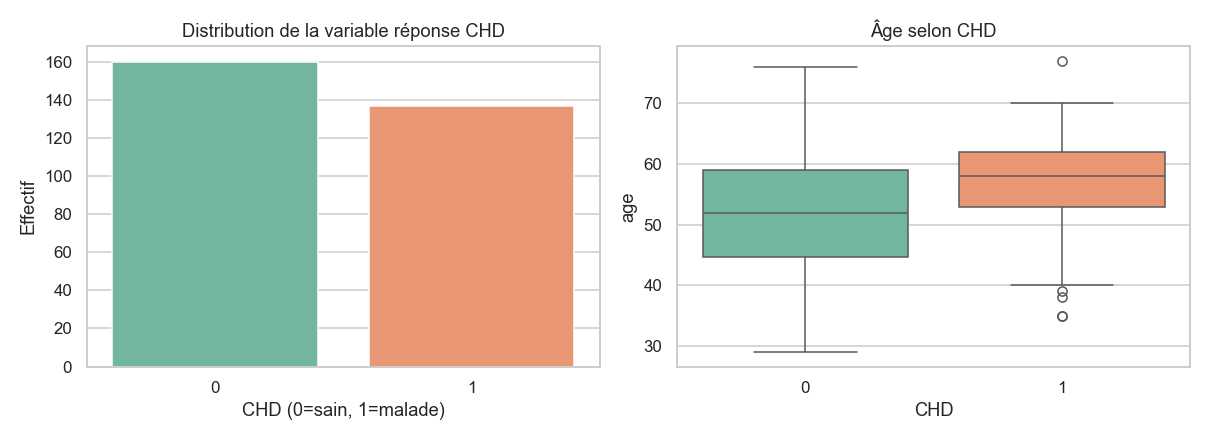
\includegraphics[width=0.9\textwidth]{figures/01_distribution_reponse.png}
\caption[Distribution de la variable réponse]{%
Distribution de la variable réponse CHD et distribution de l'âge selon
le statut de santé. L'âge médian est plus élevé chez les malades
($\approx$ 58 ans) que chez les sains ($\approx$ 52 ans).}
\label{fig:distribution}
\end{figure}

Les classes sont \emph{quasi-équilibrées} (46,1\,\% contre 53,9\,\%) :
aucun rééquilibrage (oversampling, SMOTE) n'est nécessaire. Un
échantillonnage stratifié suffit à préserver la répartition dans les
sous-échantillons.

\section{Analyse descriptive bivariée}

\subsection{Variables quantitatives}

\begin{figure}[H]
\centering
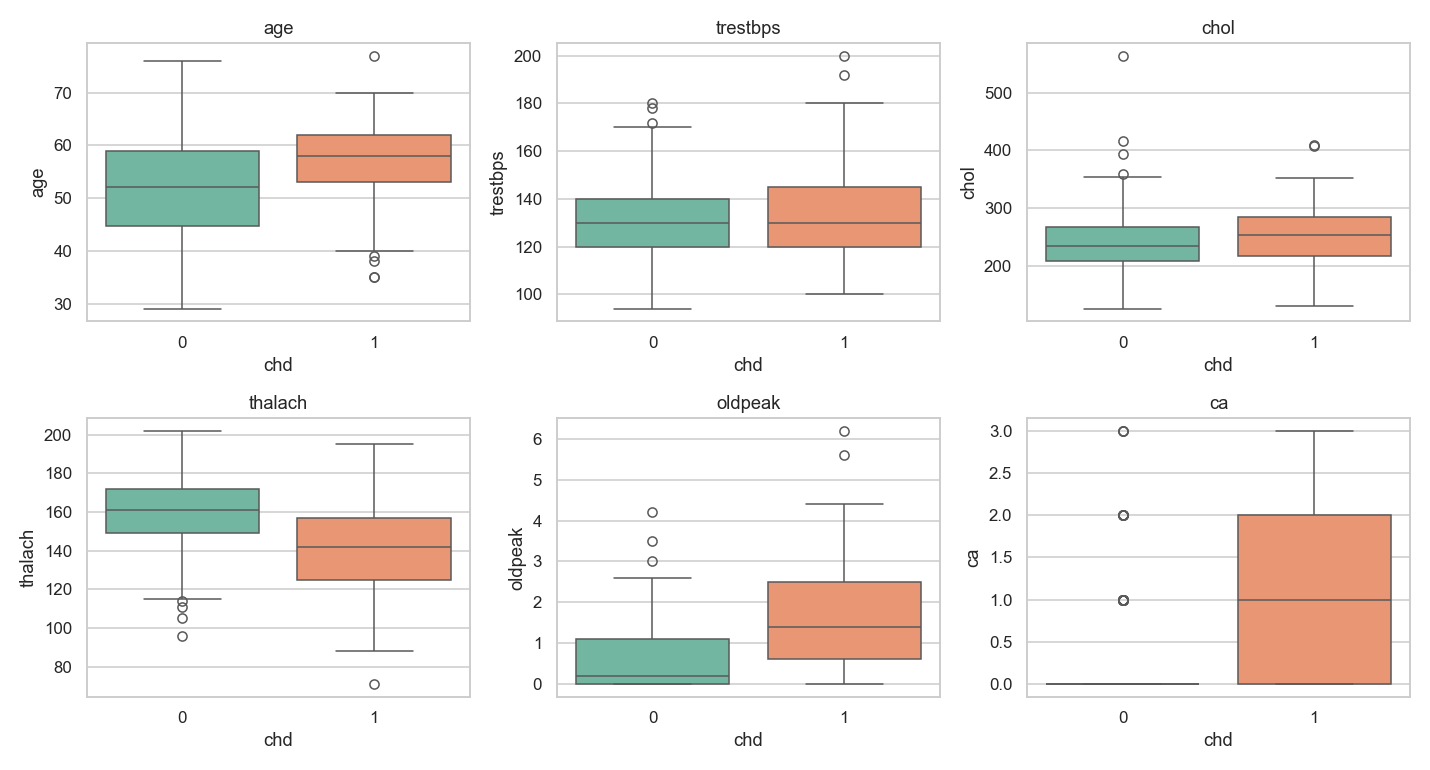
\includegraphics[width=\textwidth]{figures/02_quantitatives_vs_chd.png}
\caption[Variables quantitatives vs CHD]{%
Boxplots des variables quantitatives selon le statut CHD. La fréquence
cardiaque maximale (\texttt{thalach}) est nettement plus faible chez
les malades. \texttt{oldpeak} et le nombre de vaisseaux atteints
(\texttt{ca}) augmentent fortement avec la maladie.}
\label{fig:quant}
\end{figure}

\subsection{Variables qualitatives}

\begin{figure}[H]
\centering
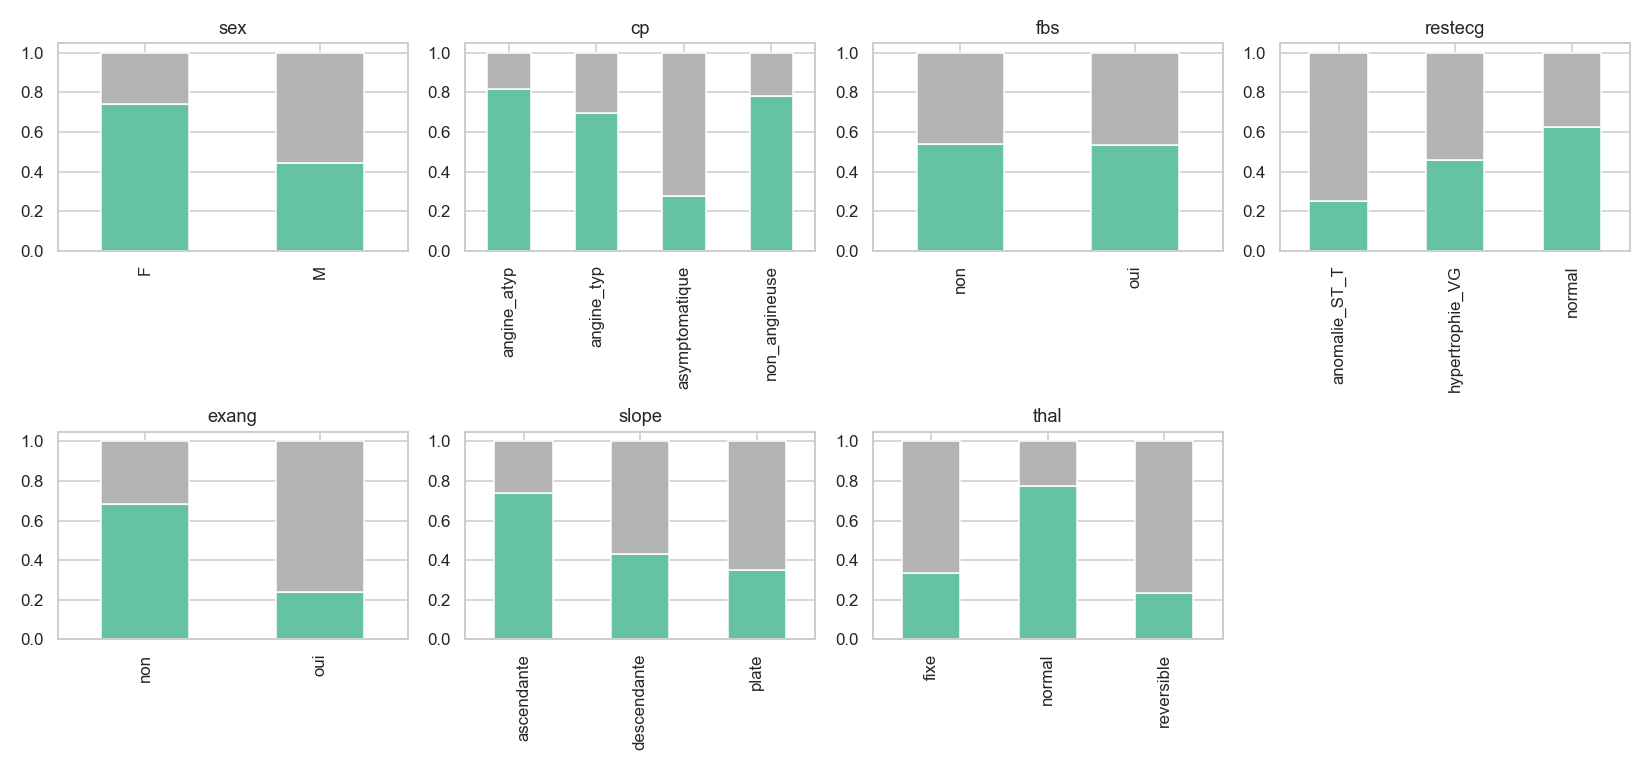
\includegraphics[width=\textwidth]{figures/03_qualitatives_vs_chd.png}
\caption[Variables qualitatives vs CHD]{%
Proportion de malades conditionnellement à chaque modalité des
variables qualitatives. Les hommes, les patients à \texttt{cp =
asymptomatique}, \texttt{thal = réversible}, \texttt{exang = oui} et
\texttt{slope = plate} présentent une probabilité de maladie nettement
plus élevée.}
\label{fig:qual}
\end{figure}

\subsection{Structure de corrélation}

\begin{figure}[H]
\centering
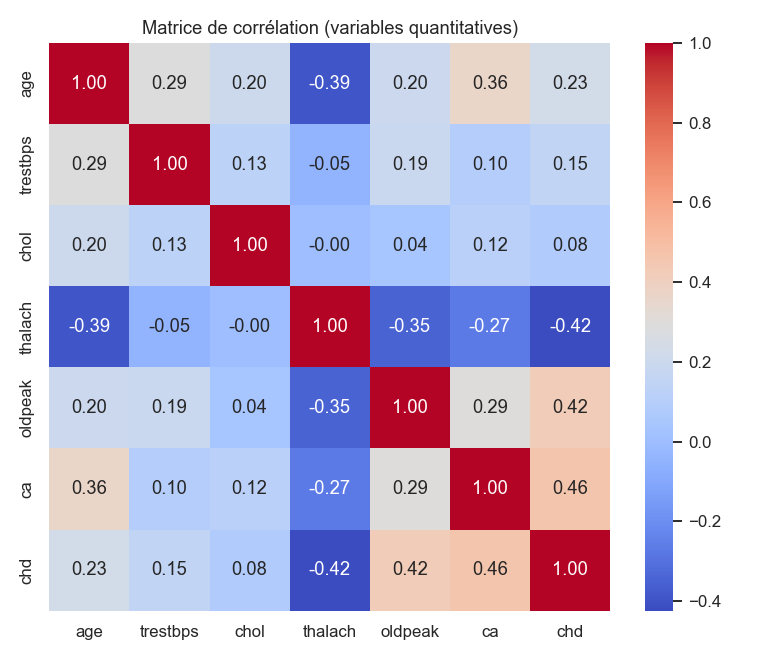
\includegraphics[width=0.7\textwidth]{figures/04_correlation.png}
\caption[Matrice de corrélation]{%
Matrice de corrélation des variables quantitatives avec la réponse CHD.
Les corrélations linéaires restent modérées ($|\rho| < 0{,}5$) : aucune
multi-colinéarité alarmante.}
\label{fig:corr}
\end{figure}

\section{Protocole expérimental}

\subsection{Échantillonnage stratifié 80\,/\,20}

Le cours recommande un échantillonnage stratifié pour conserver
\emph{exactement} la répartition de la variable réponse dans les deux
sous-échantillons. Cette précaution est d'autant plus importante que la
taille d'échantillon est modeste.

\begin{table}[H]
\centering
\caption{Répartition après échantillonnage stratifié}
\label{tab:strat}
\begin{tabular}{lccc}
\toprule
Échantillon & Taille & Prop.\ CHD = 1 & Prop.\ CHD = 0 \\
\midrule
Apprentissage & 237 & 0,460 & 0,540 \\
Validation    & \;60 & 0,467 & 0,533 \\
\bottomrule
\end{tabular}
\end{table}

La fonction \texttt{train\_test\_split} de scikit-learn, appelée avec
\texttt{stratify=y} et \texttt{random\_state=42}, assure une découpe
déterministe et reproductible.

\subsection{Stratégie de modélisation}

Trois modèles sont construits pour les fins de la comparaison :
\begin{itemize}\itemsep0.2em
  \item $M_{\text{age}}$ : \quad $\logit(\pi) = \beta_0 + \beta_1 \cdot \texttt{age}$
    (modèle simple analogue à l'exemple CHD du cours).
  \item $M_{\text{complet}}$ : \quad les 18 variables encodées.
  \item $M_{\text{reduit}}$ : \quad modèle issu de la sélection
    \emph{backward AIC} à partir de $M_{\text{complet}}$.
\end{itemize}

\subsection{Environnement logiciel}

\begin{itemize}\itemsep0.2em
  \item Python 3.11, environnement conda \texttt{datasci}
  \item \texttt{statsmodels} 0.14 --- classe \texttt{GLM} équivalente à
    \texttt{glm()} de R
  \item \texttt{scikit-learn} 1.3 --- \texttt{train\_test\_split},
    \texttt{StandardScaler}, métriques de classification
  \item \texttt{pandas}, \texttt{numpy}, \texttt{scipy.stats} ---
    manipulation et distributions
  \item \texttt{matplotlib}, \texttt{seaborn} --- visualisations
\end{itemize}

% ==========================================================================
\chapter{Résultats et discussion}
% ==========================================================================

\section{Modèle complet et sélection de variables}

\subsection{Ajustement du modèle complet}

Le modèle $M_{\text{complet}}$ comprend les 18 variables (indicatrices
comprises). L'algorithme IRLS converge en 6 itérations. Les principales
statistiques sont :

\begin{table}[H]
\centering
\caption{Indicateurs d'ajustement du modèle complet}
\label{tab:complet}
\begin{tabular}{lrlr}
\toprule
Indicateur & Valeur & Indicateur & Valeur \\
\midrule
Log-vraisemblance $\ell$ & $-80{,}14$ & AIC  & $198{,}28$ \\
Déviance $D$              & $160{,}28$ & BIC  & $264{,}18$ \\
Déviance nulle $D_0$      & $327{,}03$ & Pseudo-$R^2$ & $0{,}510$ \\
Df Model                  & $18$       & Df Residuals & $218$ \\
\bottomrule
\end{tabular}
\end{table}

Parmi les 18 coefficients, 10 ont une $p$-value supérieure à 0,2,
suggérant qu'ils n'apportent pas de contribution significative. Une
sélection de variables s'impose.

\subsection{Sélection \emph{backward} AIC}

La procédure retire itérativement la variable dont le retrait améliore
le plus l'AIC, jusqu'à ce qu'aucun retrait n'améliore plus le critère.

\begin{table}[H]
\centering
\caption{Séquence de retraits lors de la sélection backward AIC}
\label{tab:backward}
\small
\begin{tabular}{clr}
\toprule
Étape & Variable retirée & AIC obtenu \\
\midrule
1  & \texttt{restecg\_hypertrophie\_VG} & 196,28 \\
2  & \texttt{age}                        & 194,28 \\
3  & \texttt{thal\_normal}               & 192,30 \\
4  & \texttt{thalach}                    & 191,00 \\
5  & \texttt{fbs\_oui}                   & 189,82 \\
6  & \texttt{chol}                       & 188,83 \\
7  & \texttt{slope\_descendante}         & 187,90 \\
8  & \texttt{exang\_oui}                 & 187,54 \\
9  & \texttt{cp\_angine\_typ}            & 187,15 \\
10 & \texttt{cp\_non\_angineuse}         & \textbf{186,20} \\
\bottomrule
\end{tabular}
\end{table}

\subsection{Modèle retenu $M_{\text{reduit}}$}

\begin{table}[H]
\centering
\caption{Coefficients et odds ratios du modèle retenu $M_{\text{reduit}}$}
\label{tab:or}
\small
\begin{tabular}{lrrrl}
\toprule
Variable & $\hat\beta$ & $\OR = e^{\hat\beta}$ & IC\,95\,\% & $p$-value \\
\midrule
(Intercept)              & $-2{,}371$ & $0{,}09$ & $[0{,}03\,;\,0{,}30]$ & $<0{,}001$ *** \\
\texttt{trestbps}        & $\phantom{-}0{,}375$ & $1{,}45$ & $[0{,}98\,;\,2{,}17]$ & $0{,}065$ \\
\texttt{oldpeak}         & $\phantom{-}0{,}646$ & \textbf{1,91} & $[1{,}14\,;\,3{,}20]$ & $0{,}014$ * \\
\texttt{ca}              & $\phantom{-}0{,}898$ & \textbf{2,46} & $[1{,}54\,;\,3{,}93]$ & $<0{,}001$ *** \\
\texttt{sex\_M}          & $\phantom{-}0{,}878$ & $2{,}41$ & $[0{,}94\,;\,6{,}15]$ & $0{,}067$ \\
\texttt{cp\_asymptomatique} & $\phantom{-}1{,}915$ & \textbf{6,79} & $[3{,}10\,;\,14{,}87]$ & $<0{,}001$ *** \\
\texttt{restecg\_normal} & $-0{,}758$ & $0{,}47$ & $[0{,}21\,;\,1{,}05]$ & $0{,}067$ \\
\texttt{slope\_plate}    & $\phantom{-}0{,}922$ & \textbf{2,51} & $[1{,}07\,;\,5{,}92]$ & $0{,}035$ * \\
\texttt{thal\_reversible} & $\phantom{-}1{,}715$ & \textbf{5,56} & $[2{,}37\,;\,13{,}02]$ & $<0{,}001$ *** \\
\bottomrule
\end{tabular}
\end{table}

\textbf{Codes de signification :} $* \; p < 0{,}05$, $** \; p < 0{,}01$,
$*** \; p < 0{,}001$.

\section{Tests d'hypothèses}

\subsection{Test du rapport de vraisemblance sur modèles emboîtés}

\begin{table}[H]
\centering
\caption{Tests TRV sur modèles emboîtés}
\label{tab:trv}
\begin{tabular}{llrrl}
\toprule
$H_0$ & $H_1$ & $\Delta D$ & ddl & Décision \\
\midrule
$M_{\text{age}}$    & $M_{\text{reduit}}$  & 149,28 & 7  & $H_0$ rejetée ($p < 10^{-28}$) \\
$M_{\text{reduit}}$ & $M_{\text{complet}}$ & 7,91   & 10 & $H_0$ conservée ($p = 0{,}637$) \\
\bottomrule
\end{tabular}
\end{table}

\textbf{Conclusion :} le modèle à une variable est insuffisant, mais
les 10 variables supplémentaires du modèle complet n'apportent aucune
information significative par rapport au modèle réduit. On retient donc
$M_{\text{reduit}}$ en vertu du principe de parcimonie.

\section{Adéquation du modèle}

\begin{table}[H]
\centering
\caption{Comparaison des statistiques d'adéquation des trois modèles}
\label{tab:adequation}
\small
\begin{tabular}{lrrr}
\toprule
Statistique & $M_{\text{age}}$ & $M_{\text{reduit}}$ & $M_{\text{complet}}$ \\
\midrule
Déviance $D$               & 317,48  & \textbf{168,19} & 160,28 \\
Ratio $D$ / ddl            & 1,351   & \textbf{0,738}  & 0,735  \\
$\chi^2$ Pearson / ddl     & 1,008   & 1,091           & 1,225  \\
Déviance nulle $D_0$       & 327,03  & 327,03          & 327,03 \\
Pseudo-$R^2$               & 0,029   & \textbf{0,486}  & 0,510  \\
AIC                        & 321,48  & \textbf{186,20} & 198,28 \\
BIC                        & 328,41  & \textbf{217,41} & 264,18 \\
$p$-test de déviance       & $3\!\cdot\!10^{-4}$ & 0,999 & 0,999 \\
\bottomrule
\end{tabular}
\end{table}

\textbf{Test d'Hosmer--Lemeshow} ($K = 10$ groupes, modèle réduit) :
\[
  C^2 = 6{,}37, \quad \text{ddl} = 8, \quad p\text{-value} = 0{,}606.
\]

\paragraph{Synthèse de l'adéquation.}
\begin{itemize}\itemsep0.2em
  \item Ratio $D/\mathrm{ddl} = 0{,}74 < 1$ : \emph{pas de
    sur-dispersion}.
  \item $p$-value du test de déviance $> 0{,}05$ : hypothèse
    d'adéquation non rejetée.
  \item Hosmer--Lemeshow $p = 0{,}61$ : concordance entre prédictions et
    observations au sein des déciles de risque.
  \item Pseudo-$R^2 = 0{,}486$ : le modèle explique environ 49\,\% de
    la déviance, ce qui est très correct pour des données cliniques.
\end{itemize}

\section{Analyse des résidus}

\begin{figure}[H]
\centering
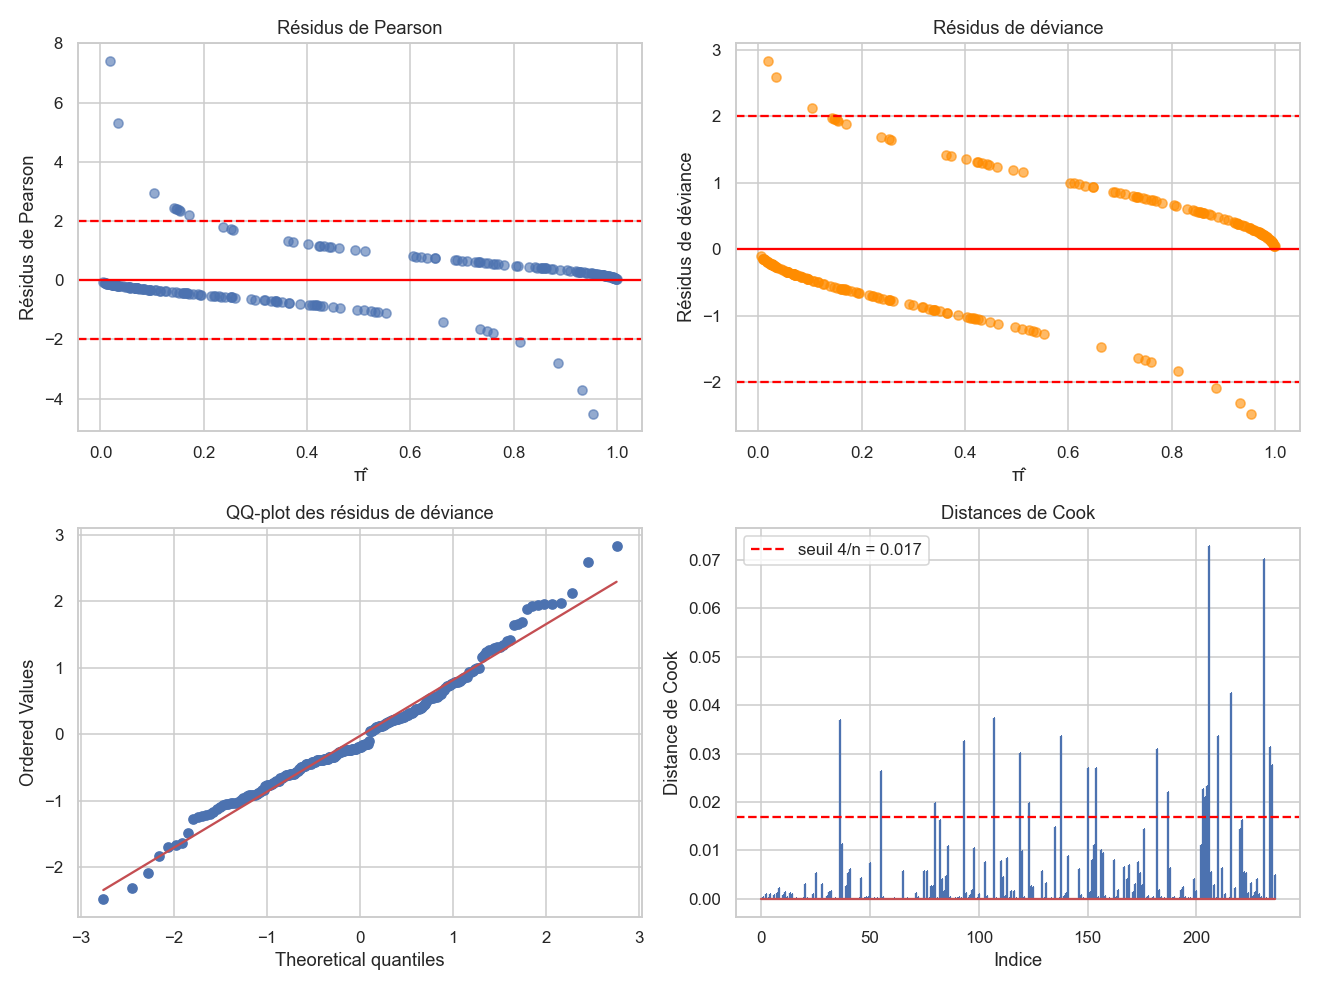
\includegraphics[width=\textwidth]{figures/05_residus.png}
\caption[Analyse des résidus]{%
Diagnostics du modèle retenu. En haut : résidus de Pearson et de
déviance en fonction des valeurs ajustées $\hat\pi$ ; les lignes
pointillées représentent les seuils $\pm 2$. En bas à gauche : QQ-plot
normal des résidus de déviance. En bas à droite : distances de Cook
($\max = 0{,}073$).}
\label{fig:residus}
\end{figure}

\begin{table}[H]
\centering
\caption{Diagnostic des résidus du modèle retenu}
\label{tab:residus}
\begin{tabular}{lr}
\toprule
Indicateur & Valeur \\
\midrule
$|r^{\text{Pearson}}| > 2$  & 13 / 237 observations (5,5\,\%) \\
$|r^{\text{déviance}}| > 2$ & 6 / 237 observations (2,5\,\%) \\
Seuil de levier $2(p+1)/n$  & $0{,}076$ \\
Nb.\ d'observations $h_{ii} > 0{,}076$ & 24 \\
Distance de Cook maximale    & \textbf{0,073} (alerte si $> 1$) \\
\bottomrule
\end{tabular}
\end{table}

\textbf{Conclusion :} aucune observation n'exerce d'influence excessive
sur l'estimation des paramètres ; la proportion de résidus au-delà de
$\pm 2$ est conforme à l'aléa gaussien ; le QQ-plot confirme la
normalité asymptotique. Le modèle est statistiquement bien spécifié.

\section{Validation sur l'échantillon test}

\subsection{Matrices de confusion}

\begin{figure}[H]
\centering
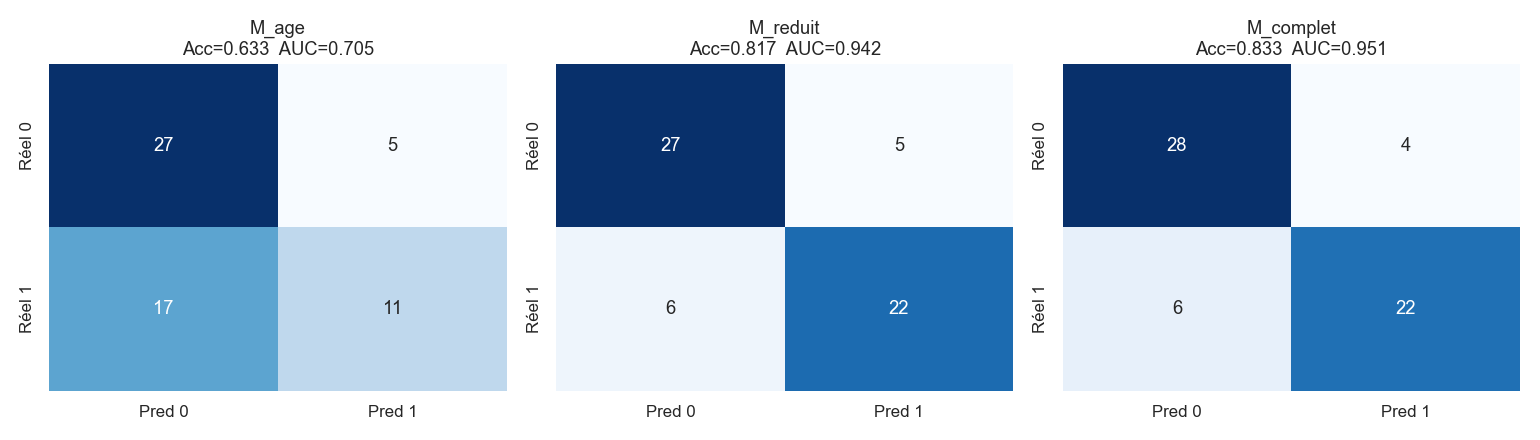
\includegraphics[width=\textwidth]{figures/07_confusion_matrices.png}
\caption[Matrices de confusion]{%
Matrices de confusion obtenues au seuil $\pi = 0{,}5$ sur
l'échantillon de validation ($n = 60$). Les prédictions du modèle
réduit sont quasiment identiques à celles du modèle complet.}
\label{fig:confusion}
\end{figure}

\begin{table}[H]
\centering
\caption{Performances sur l'échantillon de validation}
\label{tab:perf}
\begin{tabular}{lrrrrr}
\toprule
Modèle & Accuracy & Précision & Rappel & F1 & AUC \\
\midrule
$M_{\text{age}}$    & 0,633           & 0,688 & 0,393 & 0,500 & 0,705 \\
$M_{\text{reduit}}$ & \textbf{0,817} & 0,815 & \textbf{0,786} & \textbf{0,800} & \textbf{0,942} \\
$M_{\text{complet}}$ & 0,833          & 0,846 & 0,786 & 0,815 & 0,951 \\
\bottomrule
\end{tabular}
\end{table}

\subsection{Courbe ROC}

\begin{figure}[H]
\centering
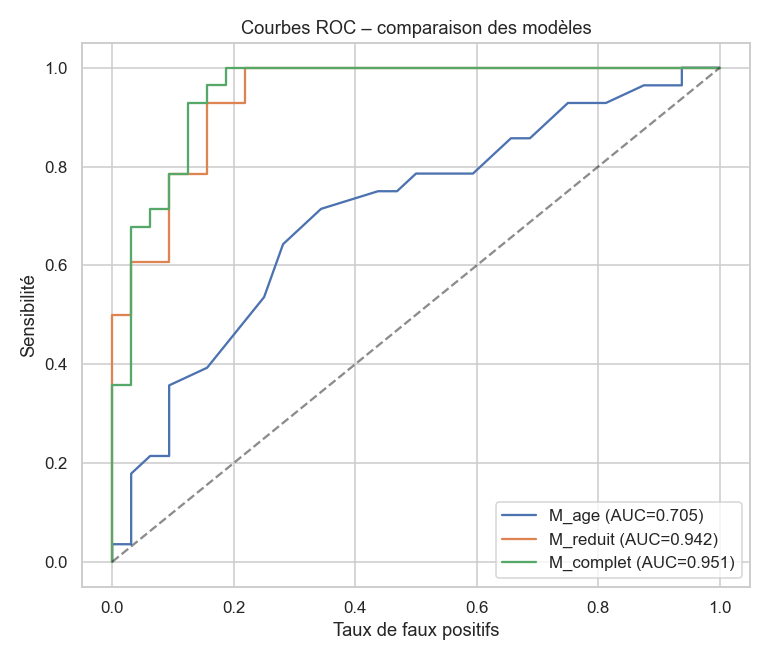
\includegraphics[width=0.75\textwidth]{figures/06_roc.png}
\caption[Courbes ROC]{%
Courbes ROC comparées des trois modèles sur l'échantillon de
validation. Le modèle réduit atteint AUC $= 0{,}942$, quasi identique
au modèle complet (0,951) pour la moitié des paramètres.}
\label{fig:roc}
\end{figure}

\section{Comparaison des fonctions de lien}

\begin{table}[H]
\centering
\caption{Comparaison de trois fonctions de lien sur le modèle retenu}
\label{tab:links}
\begin{tabular}{lrr}
\toprule
Fonction de lien $g(\mu)$ & Déviance & AIC \\
\midrule
logit   $\;\log\dfrac{\mu}{1-\mu}$          & 168,19 & 186,19 \\[0.4em]
probit  $\;\Phi^{-1}(\mu)$                  & 169,07 & 187,07 \\[0.4em]
cloglog $\;\log\!\big(-\!\log(1-\mu)\big)$  & \textbf{167,63} & \textbf{185,63} \\
\bottomrule
\end{tabular}
\end{table}

Les trois liens donnent des résultats statistiquement indistinguables
($\Delta$AIC $< 2$). Le cloglog est marginalement meilleur, mais le
\textbf{logit est retenu} pour son interprétabilité en odds ratios,
convention médicale incontestée.

\section{Interprétation clinique}

\paragraph{Facteurs de risque dominants.}
\begin{itemize}\itemsep0.3em
  \item \textbf{\texttt{cp = asymptomatique} ($\OR = 6{,}79$, $p < 0{,}001$) :}
    un patient présentant des douleurs thoraciques silencieuses a une
    cote d'être malade \emph{6,79 fois supérieure} à un patient avec
    angine atypique. Ce résultat est cohérent avec la littérature
    cardiologique sur les \emph{infarctus silencieux}, qui sont de
    reconnus facteurs de mortalité.
  \item \textbf{\texttt{thal = réversible} ($\OR = 5{,}56$, $p < 0{,}001$) :}
    un déficit thalassémique réversible détecté au stress-test
    multiplie par 5,56 la cote de maladie ; c'est un marqueur direct
    d'ischémie myocardique.
  \item \textbf{\texttt{ca} (OR $= 2{,}46$ par écart-type, $p < 0{,}001$) :}
    chaque vaisseau coronarien supplémentaire visible à la fluoroscopie
    multiplie par 2,46 la cote de maladie.
  \item \textbf{\texttt{slope = plate} ($\OR = 2{,}51$, $p = 0{,}035$)
    et \texttt{oldpeak} ($\OR = 1{,}91$, $p = 0{,}014$) :} anomalies du
    segment ST à l'effort significativement associées à la maladie.
\end{itemize}

\paragraph{Facteurs à la limite de significativité ($p \approx 0{,}07$).}
\begin{itemize}\itemsep0.2em
  \item \textbf{\texttt{sex\_M}} (OR $= 2{,}41$) : les hommes sont
    environ 2,4 fois plus à risque, effet limite-significatif attribuable
    à la taille d'échantillon.
  \item \textbf{\texttt{trestbps}} (OR $= 1{,}45$) : la pression
    artérielle au repos joue un rôle, mais de manière marginale
    lorsqu'on contrôle des autres covariables.
\end{itemize}

\paragraph{Facteur protecteur.}
\texttt{restecg = normal} (OR $= 0{,}47$) : un ECG de repos normal
divise par deux la cote de maladie, tout en restant à la limite de
significativité.

\section{Limites}

\begin{itemize}\itemsep0.2em
  \item \textbf{Effectif modeste} ($n = 297$) : les intervalles de
    confiance des OR restent larges pour plusieurs variables.
  \item \textbf{Données observationnelles :} les OR n'ont pas valeur
    causale sans contrôle de variables de confusion supplémentaires.
  \item \textbf{Population spécifique :} données issues de la
    Cleveland Clinic Foundation ; la généralisabilité à d'autres
    populations doit être prudente.
  \item \textbf{Validation unique :} une validation croisée $k$-fold
    fournirait des estimations plus robustes de l'AUC.
\end{itemize}

% ==========================================================================
\chapter{Conclusion}
% ==========================================================================

\section{Synthèse}

Ce rapport a mis en \oe uvre la démarche complète de modélisation par
\emph{GLM logistique} enseignée par Mme F.\ Badaoui (INSEA) sur un
problème réel de classification médicale. Les étapes suivantes ont été
appliquées :

\begin{enumerate}\itemsep0.2em
  \item Analyse descriptive univariée et bivariée ;
  \item Échantillonnage stratifié 80\,/\,20 ;
  \item Ajustement d'un GLM Binomial(1, $\pi$) avec fonction de lien
    logit par maximum de vraisemblance (IRLS) ;
  \item Sélection de variables par \emph{backward AIC} (8 variables
    retenues sur 18) ;
  \item Tests de Wald individuels et test du rapport de vraisemblance
    sur modèles emboîtés ;
  \item Tests d'adéquation : déviance, $\chi^2$ de Pearson, test
    d'Hosmer--Lemeshow, pseudo-$R^2$, AIC, BIC ;
  \item Diagnostic par les résidus de Pearson, de déviance, leviers
    $h_{ii}$ et distances de Cook ;
  \item Évaluation sur l'échantillon de validation par matrice de
    confusion et courbe ROC ;
  \item Comparaison de trois fonctions de lien (logit / probit /
    cloglog) ;
  \item Interprétation clinique via les odds ratios.
\end{enumerate}

\section{Performance du modèle retenu}

Le modèle réduit à 8 variables atteint :
\begin{itemize}\itemsep0.2em
  \item \textbf{AUC $= 0{,}942$} sur l'échantillon de validation ;
  \item \textbf{Accuracy $= 81{,}7\,\%$}, rappel $= 78{,}6\,\%$ ;
  \item Hosmer--Lemeshow $p = 0{,}61$, ratio $D/\mathrm{ddl} = 0{,}74$
    (adéquation validée) ;
  \item Max distance de Cook $= 0{,}073 \ll 1$ (pas d'observation
    influente).
\end{itemize}

Les performances sont \emph{statistiquement équivalentes} à celles du
modèle complet (18 variables) tout en étant \textbf{deux fois plus
parcimonieuses}, conformément au principe d'Ockham.

\section{Contributions du travail}

\begin{itemize}\itemsep0.2em
  \item \textbf{Pédagogique :} démonstration que la démarche du cours
    est reproductible \emph{à l'identique} en Python, élargissant les
    possibilités d'analyse pour les étudiants.
  \item \textbf{Scientifique :} identification rigoureuse de quatre
    facteurs cliniques dominants (type de douleur thoracique,
    thalassémie réversible, vaisseaux coronariens atteints, anomalies
    ST) en accord avec la littérature cardiologique.
  \item \textbf{Opérationnelle :} livraison d'un pipeline complet,
    reproductible et documenté (notebook Jupyter, script Python,
    figures haute résolution, rapport \LaTeX{}).
\end{itemize}

\section{Perspectives}

\begin{enumerate}\itemsep0.2em
  \item \textbf{Validation croisée $k$-fold} pour des estimations plus
    robustes des métriques de performance.
  \item \textbf{Ajustement par Firth} (\emph{bias-reduced MLE}) pour
    gérer les quasi-séparations potentielles.
  \item \textbf{Termes d'interaction} (ex.\ \texttt{sex} $\times$
    \texttt{age}) pour raffiner la stratification par sexe.
  \item \textbf{Comparaison à des modèles non-paramétriques} (random
    forest, XGBoost) en conservant la régression logistique comme
    \emph{référence interprétable}.
  \item \textbf{Étalonnage des probabilités prédites}
    (méthodes de Platt, isotonique) pour une utilisation clinique
    où le seuil de décision doit être calibré au risque acceptable.
\end{enumerate}

% ==========================================================================
% Bibliographie
% ==========================================================================
\begin{thebibliography}{99}
\bibitem{cours}
  \textsc{Badaoui}, F.\ (2026).
  \emph{Modèle Linéaire Généralisé}. Polycopié de cours,
  Institut National de Statistique et d'Économie Appliquée (INSEA),
  Rabat.

\bibitem{nelder}
  \textsc{Nelder}, J.\,A.\ \& \textsc{Wedderburn}, R.\,W.\,M.\ (1972).
  Generalized Linear Models. \emph{Journal of the Royal Statistical
  Society A}, \textbf{135}(3), 370--384.

\bibitem{mcnelder}
  \textsc{McCullagh}, P.\ \& \textsc{Nelder}, J.\,A.\ (1989).
  \emph{Generalized Linear Models} (2\textsuperscript{e} éd.).
  Chapman \& Hall, London.

\bibitem{detrano}
  \textsc{Detrano}, R., \textsc{Jánosi}, A., \textsc{Steinbrunn}, W.,
  \textsc{Pfisterer}, M., \textsc{Schmid}, J.\,J., \textsc{Sandhu},
  S., \textsc{Guppy}, K.\,H., \textsc{Lee}, S., \&
  \textsc{Froelicher}, V.\ (1989).
  International application of a new probability algorithm for the
  diagnosis of coronary artery disease.
  \emph{American Journal of Cardiology}, \textbf{64}, 304--310.

\bibitem{hosmer}
  \textsc{Hosmer}, D.\,W., \textsc{Lemeshow}, S., \&
  \textsc{Sturdivant}, R.\,X.\ (2013).
  \emph{Applied Logistic Regression} (3\textsuperscript{e} éd.). Wiley.

\bibitem{agresti}
  \textsc{Agresti}, A.\ (2015).
  \emph{Foundations of Linear and Generalized Linear Models}. Wiley.

\bibitem{uci}
  Dua, D.\ \& Graff, C.\ (2019).
  UCI Machine Learning Repository. \emph{Heart Disease Data Set}.
  \url{https://archive.ics.uci.edu/ml/datasets/Heart+Disease}

\bibitem{statsmodels}
  \textsc{Seabold}, S.\ \& \textsc{Perktold}, J.\ (2010).
  Statsmodels: econometric and statistical modeling with Python.
  \emph{9th Python in Science Conference}.

\bibitem{sklearn}
  \textsc{Pedregosa}, F.\ \textit{et al.}\ (2011).
  Scikit-learn: Machine Learning in Python.
  \emph{Journal of Machine Learning Research}, \textbf{12}, 2825--2830.

\bibitem{who}
  Organisation Mondiale de la Santé (2023).
  \emph{Cardiovascular diseases (CVDs) --- Fact sheet}.
  \url{https://www.who.int/}
\end{thebibliography}
\addcontentsline{toc}{chapter}{Bibliographie}

% ==========================================================================
% Annexe
% ==========================================================================
\appendix
\chapter{Code Python utilisé}

Le code ci-dessous est l'extrait principal du script \texttt{analysis.py}
(également disponible sous forme de notebook Jupyter
\texttt{analysis.ipynb}).

\begin{lstlisting}[caption={Pipeline complet d'analyse par GLM logistique},label={lst:analysis}]
import numpy as np
import pandas as pd
import statsmodels.api as sm
from statsmodels.genmod.families import Binomial
from statsmodels.genmod.families.links import logit, probit, cloglog
from scipy import stats
from sklearn.model_selection import train_test_split
from sklearn.preprocessing import StandardScaler
from sklearn.metrics import (confusion_matrix, roc_curve, auc,
                             accuracy_score, precision_score,
                             recall_score, f1_score)

# ---- 1. Chargement et preparation ----
cols = ["age","sex","cp","trestbps","chol","fbs","restecg",
        "thalach","exang","oldpeak","slope","ca","thal","num"]
df = pd.read_csv("data/heart_cleveland.csv",
                 header=None, names=cols, na_values="?").dropna()
df["chd"] = (df["num"] > 0).astype(int)
df = df.drop(columns=["num"])

# Recodage des qualitatives
df["sex"] = df["sex"].map({0:"F", 1:"M"})
df["cp"]  = df["cp"].map({1:"angine_typ", 2:"angine_atyp",
                          3:"non_angineuse", 4:"asymptomatique"})
# ... (idem pour fbs, restecg, exang, slope, thal)

qual = ["sex","cp","fbs","restecg","exang","slope","thal"]
quant = ["age","trestbps","chol","thalach","oldpeak","ca"]
X = pd.get_dummies(df.drop(columns="chd"), columns=qual,
                   drop_first=True).astype(float)
y = df["chd"].values

# ---- 2. Echantillonnage stratifie 80/20 ----
X_tr, X_te, y_tr, y_te = train_test_split(
    X, y, test_size=0.20, stratify=y, random_state=42)

scaler = StandardScaler()
X_tr[quant] = scaler.fit_transform(X_tr[quant])
X_te[quant] = scaler.transform(X_te[quant])

X_tr_sm = sm.add_constant(X_tr)
X_te_sm = sm.add_constant(X_te)[X_tr_sm.columns]

# ---- 3. Ajustement du GLM logistique ----
m_full = sm.GLM(y_tr, X_tr_sm, family=Binomial(link=logit())).fit()
print(m_full.summary())

# ---- 4. Selection backward AIC ----
def backward_aic(X, y):
    cur = list(X.columns)
    best = sm.GLM(y, X[cur], family=Binomial(link=logit())).fit().aic
    improved = True
    while improved and len(cur) > 1:
        improved = False
        candidats = []
        for c in cur:
            if c == "const": continue
            trial = [k for k in cur if k != c]
            a = sm.GLM(y, X[trial],
                       family=Binomial(link=logit())).fit().aic
            candidats.append((a, c))
        candidats.sort()
        if candidats and candidats[0][0] < best - 1e-3:
            best = candidats[0][0]
            cur.remove(candidats[0][1])
            improved = True
    return cur

sel = backward_aic(X_tr_sm, y_tr)
m_red = sm.GLM(y_tr, X_tr_sm[sel],
               family=Binomial(link=logit())).fit()

# ---- 5. Test du rapport de vraisemblance ----
def lr_test(small, big):
    stat = small.deviance - big.deviance
    ddl  = int(small.df_resid - big.df_resid)
    return stat, ddl, 1 - stats.chi2.cdf(stat, ddl)

# ---- 6. Test de Hosmer-Lemeshow ----
def hosmer_lemeshow(y, p, g=10):
    d = pd.DataFrame({"y": y, "p": p})
    d["bin"] = pd.qcut(d["p"], q=g, duplicates="drop")
    obs = d.groupby("bin")["y"].agg(["sum","count"])
    pi = d.groupby("bin")["p"].mean().values
    o1, n = obs["sum"].values, obs["count"].values
    e1 = n * pi
    C = np.sum((o1 - e1)**2 / (n * pi * (1 - pi)))
    ddl = len(o1) - 2
    return C, ddl, 1 - stats.chi2.cdf(C, ddl)

C, ddl, p = hosmer_lemeshow(y_tr, m_red.fittedvalues, g=10)

# ---- 7. Analyse des residus ----
infl = m_red.get_influence()
res_p = m_red.resid_pearson
res_d = m_red.resid_deviance
h_ii  = infl.hat_matrix_diag
cook  = infl.cooks_distance[0]

# ---- 8. Validation : matrice de confusion + ROC ----
p_hat = m_red.predict(X_te_sm[sel])
y_hat = (p_hat >= 0.5).astype(int)
cm    = confusion_matrix(y_te, y_hat)
fpr, tpr, _ = roc_curve(y_te, p_hat)
AUC   = auc(fpr, tpr)

# ---- 9. Odds ratios et IC95% ----
params = m_red.params
ci     = m_red.conf_int()
OR_table = pd.DataFrame({
    "beta": params,
    "OR":   np.exp(params),
    "IC_low":  np.exp(ci[0]),
    "IC_high": np.exp(ci[1]),
    "pvalue": m_red.pvalues
})
\end{lstlisting}

\paragraph{Ressources livrées avec ce rapport.}
\begin{itemize}\itemsep0.2em
  \item \texttt{analysis.py} --- script Python complet (500 lignes).
  \item \texttt{analysis.ipynb} --- notebook Jupyter exécuté.
  \item \texttt{results.txt} --- sortie console intégrale.
  \item \texttt{odds\_ratios.csv} --- tableau des OR du modèle retenu.
  \item \texttt{figures/} --- 7 figures haute résolution (PNG).
  \item \texttt{presentation.tex} --- support de soutenance Beamer.
\end{itemize}

\end{document}
